% *******************************************************************************
\chapter{Mean Shift}\label{ch:mean_shift}
% *******************************************************************************
In low level computer vision tasks like filtering, segmentation or
edge detection, the analysis of data is often not done on the original
images.  Features like colors are rather projected into a feature
space where they can be more easily analyzed. The analysis of the
feature space can find interesting attributes of the image like edges
or segments.

The feature space has to be smoothed before analysis. Feature spaces
originate from real images therefore they are composed of several
components from different distributions. The basic approach of a
mixture model, a mixture model is a probabilistic model for density
estimation using a mixture distribution, is not efficient enough to
estimate the density satisfactorily of such complex, arbitrarily
comprised densities. The discontinuity preserving smoothing is
therefore accomplished with kernel based density estimators. Kernel
based density estimators are making no assumptions about densities and
hence can estimate arbitrary densities.

The maxima of a feature space correspond to the searched components
like the edges of an image. Gradient based methods of feature space
analysis are using gradients of the probability density function to
find the maxima. Such methods are complex because they need among
other things a estimation of the probability of density.

Mean shift is an alternative to the gradient based methods as it is
easier to calculate then to estimate the probability of density and
then to calculate the gradient. The mean shift vector points to the
same direction as the gradient of gradient based methods. Furthermore
the \emph{mean shift} vector has a adaptive size and is non
parametric. There is no need to supply a step size compared to the
other methods. Mean shift a robust approach toward feature space
analysis was originally introduced by \citeauthor{citeulike:462300}
\citep{citeulike:462300}.

\section{Density Estimation} % (fold)
\label{sec:density_estimation}
In probability and statistics it is known that for different tasks
there exist more or less suitable features. In
\citeauthor{citeulike:167581} \citep{citeulike:167581} are giving an
example of a classification of two different fish types. Features like
the length and brightness are there observed that fit for the task. It
is of course possible to find more descriptive features for the fish
like the amount of finns but in image processing it would be very
expensive and difficult to count such feature. In image analysis
specially in real time applications it is important to find suitable
features for the task, but also features which are easily visually
identified. Color observations are because of their simplicity and for
the eye easily to gather important features. The color features can
have components from the \gls{RGB} or gray value color
space. Furthermore there are several other color spaces that could be
observed like the \gls{HSV} or the \gls{LUV} color space with one
luminance and two chromatic components. The \gls{LUV} color space is
often used in computer graphics because of its attribute to be a
perceptually uniform color space.

With a finite set of observations follows a finite feature space. The
main point of \emph{mean shift} is to find the maxima in the feature
space. The maxima of a feature space are all important for \emph{mean
  shift} applications (filtering, segmentation, \ldots) as the
distributions or discontinuities map to clusters or edges of the
image.

The \emph{mean shift} method is based on the gradient method. For the
gradient estimation a function is upon estimations of discrete
observations in the feature space. For this kernel density estimators
are used also known as \emph{Parzen Window} method.

\section{Kernel Density Estimation} % (fold)
\label{sec:kernel_density_estimation}
Kernel density estimation is a method to estimate an unkown density
distribution with finite observations of a point in the sample space.
The result of such a procedure is a probability density function that
describes the density of probability at each point in the sample
space. To estimate the density of a point $x = { x_1, \ldots , x_d,
  \ldots , x_D} \in \mathbb{R}^D$ in a $D$ dimensionl feature space,
$N$ observations $x_1^N$ with $x_N \in \mathbb{R}^D$ within a search
window that is centered around point $x$ have to be observed. The
search window with radius $h$ is the bandwidth of the used kernel. The
probability density in point $x$ is the mean of probability densities
that are centered in the $N$ observations $x_1^N$.

The effect of different bandwidth parameters $h$ (search window
radius) is shown in \autoref{fig:window_radius}. The example shows a
kernel density estimation with five observations $x = {5, 1, -1, -4,
  -5}$ and a gaussian kernel. The total density estimation is the sum
of each kernel at a observation, here shown for three bandwidths. With
bigger bandwidth $h$ the density estimation becomes smoother.

\begin{figure}[ht]
  \centering

  \pgfplotsset{every axis x label/.style={at={(1,0)}, above}}
  \pgfplotsset{every axis y label/.style={at={(0,1)}, left}}


  \pgfplotstableread{Plots/gauss_07.data}\tableA
  \pgfplotstableread{Plots/gauss_10.data}\tableB
  \pgfplotstableread{Plots/gauss_20.data}\tableC

  \subfloat[$h=0.7$]{
    \begin{tikzpicture}
      \begin{axis}[
        smooth,
        % stack plots=y,
        % area style,
        % ybar, bar width=10pt,
        % line width=0.7pt, %0.5pt default
        width=0.32\textwidth,
        height=3.5cm,
        % xtick={128,384,...,2688},
        ytick={0,0.2,0.4,0.6,0.8},
        axis x line=bottom,
        axis y line=left,
        % xmin=-1, xmax=1, 
        ymin=0, ymax=1.0,
        xlabel=$x$,
        ylabel=$y$,
        enlarge x limits=0.1,
        % ymajorgrids
        ]
        
        \addplot[color=pl0, mark=none] table[x=X,y=Y5] from \tableA;
        \addplot[color=pl1, mark=none] table[x=X,y=Y1] from \tableA;
        \addplot[color=pl2, mark=none] table[x=X,y=Y_1] from \tableA;
        \addplot[color=pl3, mark=none] table[x=X,y=Y_4] from \tableA;
        \addplot[color=pl4, mark=none] table[x=X,y=Y_5] from \tableA;
        \addplot[color=pl5, mark=none] table[x=X,y=SUMME] from \tableA;
        

      \end{axis}
    \end{tikzpicture}
    \label{fig:h07}
	}%
  \qquad \subfloat[$h=1.0$]{
    \begin{tikzpicture}
      \begin{axis}[
        smooth,
        % stack plots=y,
        % area style,
        % ybar, bar width=10pt,
        % line width=0.5pt, %default
        width=0.32\textwidth,
        height=3.5cm,
        % xtick={128,384,...,2688},
        ytick={0,0.2,0.4,0.6,0.8},
        axis x line=bottom,
        axis y line=left,
        % xmin=-1, xmax=1, 
        ymin=0, ymax=1.0,
        xlabel=$x$,
        ylabel=$y$,
        enlarge x limits=0.1,
        % ymajorgrids
        ]
        
        \addplot[color=pl0, mark=none] table[x=X,y=Y5] from \tableB;
        \addplot[color=pl1, mark=none] table[x=X,y=Y1] from \tableB;
        \addplot[color=pl2, mark=none] table[x=X,y=Y_1] from \tableB;
        \addplot[color=pl3, mark=none] table[x=X,y=Y_4] from \tableB;
        \addplot[color=pl4, mark=none] table[x=X,y=Y_5] from \tableB;
        \addplot[color=pl5, mark=none] table[x=X,y=SUMME] from \tableB;
        

      \end{axis}
    \end{tikzpicture}
    \label{fig:h10}}%
  \qquad \subfloat[$h=2.0$]{
    \begin{tikzpicture}
      \begin{axis}[
        smooth,
        % stack plots=y,
        % area style,
        % ybar, bar width=10pt,
        % line width=0.5pt, %default
        width=0.32\textwidth,
        height=3.5cm,
        % xtick={128,384,...,2688},
        ytick={0,0.2,0.4,0.6,0.8},
        axis x line=bottom,
        axis y line=left,
        % xmin=-1, xmax=1, 
        ymin=0, ymax=1.0,
        xlabel=$x$,
        ylabel=$y$,
        enlarge x limits=0.1,
        % ymajorgrids
        ]
        
        \addplot[color=pl0, mark=none] table[x=X,y=Y5] from \tableC;
        \addplot[color=pl1, mark=none] table[x=X,y=Y1] from \tableC;
        \addplot[color=pl2, mark=none] table[x=X,y=Y_1] from \tableC;
        \addplot[color=pl3, mark=none] table[x=X,y=Y_4] from \tableC;
        \addplot[color=pl4, mark=none] table[x=X,y=Y_5] from \tableC;
        \addplot[color=pl5, mark=none] table[x=X,y=SUMME] from \tableC;
        

      \end{axis}
    \end{tikzpicture}
    \label{fig:h20}}%

  \caption{Effect of bandwidth selection}
  \label{fig:window_radius}
\end{figure}


Kernel density estimation is a non parametric method, although some
parameters exists like the search window radius. Non parametric
methods are making no assumptions about the density of
probabilities. The strenght of such methods is that they are not
limited to just one probability but they can deal with arbitrary
coupled/joined probabilities. With an unfinite number of observations
the non parametric methods can reconstruct the density of the original
probabilities.

To derive the kernel density estimator in point $x \in \mathbb{R}^D$
first of all some definitions have to be made. Let $x$ be a random
variable and $N$ observations $x_1^N$ with $x_n \in \mathbb{R}^D$
given. The kernel density estimator $\hat{f}(x)$ in a point $x \in
\mathbb{R}^D$, with a kernel $K(x)$ and a $D \times D$ bandwith matrix
$\mathbf{H}$ is
\begin{equation}\label{eq:kernel0}
  \hat{f}(x) = \frac{1}{N} \sum_{n = 1}^N K_{\mathbf{H}}\left( x-x_n \right)
\end{equation} 
where
\begin{equation}\label{eq:kernel1}
  K_{\mathbf{H}}(x) = \frac{1}{\sqrt{|\mathbf{H}|}}K \left( \frac{x - x_n}{h} \right)
\end{equation} 

Since a full parametrized matrix $\mathbf{H}$ would lead to very
complex estimates only a single bandwidth parameter, the window radius
will be regarded. With the simplification $\mathbf{H} = h^2
\mathbf{I}$ the \autoref{eq:kernel0} can be written as
\begin{equation}\label{eq:kernel2}
  \hat{f}(x) = \frac{1}{Nh^D}\sum_{n=1}^N K\left( \frac{x - x_i}{h} \right).
\end{equation}

The kernel density estimator is valid for several kernels and
successive considerations will deal with several kernel the
\autoref{eq:kernel2} will be formated into a more generic form. For
this transformation the definition of a kernel and profile of the
kernel is needed. The following definition of a kernel and its profile
is from \citeauthor{citeulike:2522867} \citep{citeulike:2522867}. The
norm $\lVert x \rVert$ of $x$ is a non negative number so that $\lVert
x \rVert^2 = \sum_{d = 1}^D|x_d|^2$.  A $K:\mathbb{R}^D \rightarrow
\mathbb{R}$ is a known as a kernel, when there is a function $k:[0,
\infty] \rightarrow \mathbb{R}$ the profile of the kernel, so that
\begin{equation}\label{eq:kernel3}
  K(x)=c_{k,d}k(\lVert x \rVert^2)
\end{equation}
where $K$ is radial symmetric, where $k$ is non negativ, not
increasingly and piecewise continuous with $\int_0^{\infty} k(r) dr <
\infty$. $c_{k,D}$ is a positive normalization constant so that $K(x)$
integrates to $1$.

Now the kernel density estimator from \autoref{eq:kernel2} can be
transformed into a new equation. The two indices $K$ and $h$ are
representing which kernel and which radius are used for the density
estimator. With the profile notation $k$, where \autoref{eq:kernel2}
is inserted into \autoref{eq:kernel1}, the \autoref{eq:kernel2} is
transformed to
\begin{equation}\label{eq:kernel4}
  \hat{f}_{h,K}(x) = \frac{c_{k,D}}{Nh^d}
  \sum_{n = 1}^N k\left(\left\lVert \frac{x-x_n}{h} \right\rVert^2\right)
\end{equation}



\section{Kernel and their Properties} % (fold)
\label{sec:kernel_properties}
The following section will introduce three univariate profiles and
their associated multivariate radial symmetric kernels.

From the Epanechnikov profile
\begin{equation}\label{eq:epa}
  k_E{x} = \begin{cases}
    1 - x &  0 \leq x \leq 1\\
    0 & x > 1
  \end{cases}, x \in \mathbb{R}
\end{equation}
follows a radial symmetric kernel
\begin{equation}\label{eq:epak}
  K_E(x) = \begin{cases}
    \frac{1}{2}c_D^{-1}(D+2)(1-\lVert x \rVert^2) &  \lVert x \rVert \leq 1 \\
    0 & \mathit{otherwise}
  \end{cases}, x \in \mathbb{R}^D
\end{equation}

where $c_D$ is the Volume of the $D$ dimensional globe. The
epanechnikov kernel is used often as it minimizes the \gls{MISE}
\citep{citeulike:5813637}. The \autoref{fig:epan} shows the
epanechnikov kernel. The dervative of the kernel is a uniform profile.



\begin{figure}[ht]
  \centering

  \pgfplotsset{every axis x label/.style={at={(1,0)}, below}}
  \pgfplotsset{every axis y label/.style={at={(0,1)}, left}}

  \subfloat[Epanechnikov]{
    \begin{tikzpicture}
      \begin{axis}[
        % smooth,
        % stack plots=y,
        % area style,
        % ybar, bar width=10pt,
        % line width=0.5pt, %default
        width=0.32\textwidth,
        height=3.5cm,
        % xtick={128,384,...,2688},
        ytick={0,0.4,0.8},
        axis x line=bottom,
        axis y line=left,
        xmin=-1, xmax=1, 
        ymin=0, ymax=1.0,
        xlabel=$x$,
        ylabel=$y$,
        enlarge x limits=0.15,
        % ymajorgrids
        ]
        
        \addplot[color=pl0] expression[domain=-1:1] {3/4*(1-x*x)};

      \end{axis}
    \end{tikzpicture}
    \label{fig:epan}
  } \qquad \subfloat[Gaussian]{

    \begin{tikzpicture}
      \begin{axis}[
        % smooth,
        % stack plots=y,
        % area style,
        % ybar, bar width=10pt,
        width=0.32\textwidth,
        height=3.5cm,
        % xtick={128,384,...,2688},
        axis x line=bottom,
        axis y line=left,
        xmin=-3, xmax=3, 
        ymin=0, ymax=0.5,
        xlabel=$x$,
        ylabel=$y$,
        enlarge x limits=0.15,
        % ymajorgrids
        ]
        
        \addplot[color=pl0] expression[domain=-3:3]
        {1/sqrt(2*3.14)*exp((-1/2)*x*x)};

      \end{axis}
    \end{tikzpicture}
    \label{fig:gaus}} \qquad \subfloat[Uniform]{


    \begin{tikzpicture}
      \begin{axis}[
        % smooth,
        % stack plots=y,
        % area style,
        % ybar, bar width=10pt,
        width=0.32\textwidth,
        height=3.5cm,
        % xtick={128,384,...,2688},
        axis x line=bottom,
        axis y line=left,
        xmin=-1, xmax=1, 
        ymin=0, ymax=1.2,
        xlabel=$x$,
        ylabel=$y$,
        enlarge x limits=0.15,
        % ymajorgrids
        mark size=0.01pt ]
        
        \addplot+[const plot,color=pl0] coordinates { (-1,0) (-1,0.5) (1,0.5)
          (1,0) };
      \end{axis}
    \end{tikzpicture}

    \label{fig:uni}}%

  \caption{Kernel density estimators}
  \label{fig:kernels}
\end{figure}

From the normal profile
\begin{equation}\label{eq:nml}
  k_N(x) = exp \left( - \frac{1}{2} x \right) \textrm{ where } x \geq 0, x \in \mathbb{R}
\end{equation}
follows the normal kernel
\begin{equation}\label{eq:nmlk}
  K_N(x) = (2\pi)^{-D/2}exp\left( -\frac{1}{2} \lVert x \rVert^2 \right), x \in \mathbb{R}.
\end{equation}
The normal distribution as every other kernel with infinite support,
is often capped for finite support. Finite support is important for
the convergence. Capping the normal kernel can be accomplished by
multiplying it by a uniform kernel where the inner part of the normal
kernel is cut out and weighted with $1$ and the outer part is set to
$0$. The derivative of the normal profile is again a normal profile.

From the uniform profile
\begin{equation}\label{eq:unf}
  k_U(x) = \begin{cases}
    1 &  0 \leq x \leq 1\\
    0 & \mathit{otherwise}
  \end{cases}, x \in \mathbb{R}
\end{equation}
follows the uniform kernel
\begin{equation}\label{eq:unfk}
  K_U(x) = \begin{cases}
    1 &  \lVert x \rVert  \leq 1\\
    0 & \mathit{otherwise}
  \end{cases}, x \in \mathbb{R}^D
\end{equation}

which is a hyper unit ball in the origin.

Assuming that a derivative of a profile $k(x)$ exists for all $x \in
[0, \infty)$, follows a new profile $g(x)$. Now a new kernel $G(x)$
can be defined as
\begin{equation}\label{eq:shadowk}
  G(x) = c_{g,D}g(\lVert x \rVert^2)
\end{equation}
where $c_{g,D}$ a normalizing constant and $K(x)$ the \emph{shadow
  kernel} of $G(x)$. The term \emph{shadow kernel} was introduced in
the context of mean shift in \citep{citeulike:2522867}. The mean shift
vector of a kernel points to the same direction as the gradient of the
shadow kernel (See \autoref{sub:gradient_estimator}).



\section{Mean Shift} % (fold)
\label{sec:mean_shift}
In gradient based methods first the gradient s calculated and then the
kernel is shifted by a vector with a specific length in direction of a
maximum of the probability. The magnitude/length that is the step size
of the vector has to be chosen. The problem of such gradient based
methods is the choice of a suitable step size. The run time of such
algorithms depends heavily on the right choice of the step size. If
the step size is too large the algorithm diverges and choosing a too
small step size the algorithm becomes very slow. Convergence is only
guaranteed for infinitesimal step sizes. There are several complex
procedures for finding the right step size, see
\citeauthor{citeulike:462300} \citep{citeulike:462300}.

In the case of mean shift there are no additional procedures needed to
choose the step size. The magnitude/length of the mean shift vector is
the step size which is adaptive regarding the local gradient of the
density of probability.  Because of this adaptive nature the mean
shift algorithm converges (Proof see \citeauthor{citeulike:462300}
\citep{citeulike:462300}).

The advantage of the mean shift method contrary to gradient based
methods is that the step size has not to be chosen by hand and the
gradient has not to be calculated. It can be shown that the mean shift
vector is pointing to the same direction as the gradient and that it
moves along the gradient to the maxima that can be seen in
\autoref{eq:ms7}. Hence it is sufficient to calculate the more
efficient mean shift vector rather than the gradient.

Given are $N$ $D$-dimensional observer feature vectors $x_1^N$ with
$x_n \in \mathbb{R}^D$ and a kernel $G$ at the point $x = {x_1, \ldots
  , x_d, \ldots , x_D} \in \mathbb{R}^D$ in the feature space with
search window radius $h$ is
\begin{equation}\label{eq:ms0}
  m_{h,G}(x) = \frac{\sum_{i=1}^n x_i g\left(\left\lVert \frac{x - x_i}{h}
      \right\rVert^2\right)}{\sum_{i=1}^n g\left(\left\lVert \frac{x - x_i}{h}
      \right\rVert^2\right)} -x
\end{equation}
the $D$-dimensional \textit{mean shift} vector. The $N$ observations
are weighted by the means of kernel $G$, summed and normalized with
the total sum.  The \emph{shift} is the difference between the
weighted \emph{mean} and $x$, thus the name \emph{mean shift}.

As pointed out in \autoref{sec:kernel_density_estimation} the main
objective of density estimation is to efficiently find the maxima of a
distribution in feature space. The maxima of a function $f$ are
located at the positions where the gradient $\nabla f(x) = 0$. With
the above stated attribute that the \emph{mean shift} vector always
moves along the direction of the gradient, it is a elegant solution
for finding the maxima of a distribution without estimating the
density.

\subsection{Density Gradient Estimation} % (fold)
\label{sub:gradient_estimation}
The usage of a differentiable kernel allows one to write the density
gradient estimator as the gradient of the density estimator

\begin{equation}\label{eq:gradest}
  \hat{\nabla} f_{h,K}(x) \equiv \nabla \hat{f}_{h,K}(x) = 
  \frac{2_{C_{k,D}}}{Nh^{D+2}}%
  \sum_{n = 1}^N (x - x_n)k' 
  \left( \left\lVert \frac{x - x_n}{h} \right\rVert^2 \right)
\end{equation}

where the inner part and a part of the prefactor originate from the
differentiation of $k\left( \left\lVert \frac{x - x_n}{h} \right\rVert
\right)$

\begin{equation}\label{eq:kerndiff}
  \begin{split}
    \frac{\delta}{\delta x} k\left( \left\lVert \frac{x - x_n}{h}
      \right\rVert^2 \right) & = \left( \left\lVert \frac{x - x_n}{h}
      \right\rVert \right)' k'\left( \left\lVert \frac{x - x_n}{h}
      \right\rVert^2 \right) \\ & = 2 \left( x - x_n \right) \left(
      \frac{1}{h} \right) k'\left( \left\lVert \frac{x - x_n}{h}
      \right\rVert^2 \right) \\ & = \frac{2}{h^2}(x - x_n) k'\left(
      \left\lVert \frac{x - x_n}{h} \right\rVert^2 \right).
  \end{split}
\end{equation}

Using $g(x) = -k'(x)$ and with \autoref{eq:shadowk} a new kernel
$G(x)$ with profile $g(x)$ can be defined. Transforming
\autoref{eq:gradest} with the new profile $g(x)$ the gradient of the
density estimator becomes
\begin{subequations}
  \begin{align}
    \hat{\nabla} f_{h,K}(x) & = \frac{2c_{k,D}}{Nh^{D+2}}\sum_{i=1}^N
    \left(x_n - x\right)g\left(\left\lVert \frac{x - x_n}{h}
      \right\rVert^2\right) \label{eq:gradest1}\\ & =
    \frac{2c_{k,D}}{Nh^{D+2}} \left[ \sum_{n=1}^N g\left(\left\lVert
          \frac{x - x_n}{h} \right\rVert^2\right) \right] \left[
      \frac{\sum_{i=1}^N x_i g\left(\left\lVert \frac{x - x_n}{h}
          \right\rVert^2\right)}{\sum_{n=1}^N g\left(\left\lVert
            \frac{x - x_n}{h} \right\rVert^2\right)} - x \right].
    \label{eq:gradest2}
  \end{align}
\end{subequations}

The first term of \autoref{eq:gradest2} conforms with the density
estimator $\hat{f}_{h,G}(x)$ for kernel $G$ (compare with
\autoref{eq:kernel4} for kernel $K$) except for a factor whereas the
second term is the difference between the center of the, with kernel
$G$ weighted center of observation and the center $x$ of the kernel
window which conforms to the \emph{mean shift} vector from
\autoref{eq:ms0}.  To localize the maxima with \emph{mean shift}, the
maxima are the roots of the gradient, it firstly has to be shown that
the \emph{mean shift} vektor is moving along the direction of the
gradient. Inserting $\hat{f}_{h,G}(x)$ and $m_{h,G}(x)$ into
\autoref{eq:gradest2} follows
\begin{equation}\label{eq:ms1}
  \hat{\nabla} f_{h,K}(x) = \frac{2c_{k,D}}{h^2c_{g,D}} 
  \hat{f}_{h,G}(x)m_{h,G}(x)
\end{equation}
transformed to $m_{h,G}(x)$ follows
\begin{equation}\label{eq:ms2}
  m_{h,G}(x) = \frac{1}{2}h^2 c 
  \frac{\hat{\nabla} f_{h,K}(x)}{\hat{f}_h,G(x)}, \textrm{ whereas } 
  c = \frac{c_{g,D}}{c_{k,D}}.
\end{equation}

The denominator of \autoref{eq:ms2} is the normalizing factor that
originates from the density estimator with kernel $G$ in $x$ and the
numerator is the gradient density estimator with kernel $K$. In fact
the \emph{mean shift} vector is proportional to the gradient which
means it is adaptive. Kernel $K$ is the shadow kernel of kernel
$G$. The term shadow kernel was firstly introduced by
\citeauthor{citeulike:2522867} \citep{citeulike:2522867}.

Let be
\begin{equation}\label{eq:msi}
  mi_{h,K}(x) = \frac{\sum_{i=1}^n x_i k\left(\left\lVert \frac{x - x_i}{h}
      \right\rVert^2\right)}{\sum_{i=1}^n k\left(\left\lVert \frac{x - x_i}{h}
      \right\rVert^2\right)} -x
\end{equation}
the $D$-dimensional mean of the observations $x_1^N$ from
$\mathbb{R}^D$ weighted with kernel $K$ and a window radius $h$. Then
is $K$ the shadow kernel to kernel $G$ if the \emph{mean shift} vector
with kernel $G$
\begin{equation}\label{eq:msi2}
  m_{h,G}(x) = mi_{h,G}(x) - x = 
  \frac{\sum_{i=1}^n x_i g\left(\left\lVert \frac{x - x_i}{h}
      \right\rVert^2\right)}{\sum_{i=1}^n g\left(\left\lVert \frac{x - x_i}{h}
      \right\rVert^2\right)} -x
\end{equation}
lies in the gradient density estimator direction with kernel $K$
\begin{equation}\label{eq:msi3}
  \hat{f}_{h,K}(x) = \frac{c_{k,D}}{Nh^d}
  \sum_{n = 1}^N k\left(\left\lVert \frac{x-x_n}{h} \right\rVert^2\right)
\end{equation}

In the following sections gradients will not more be considered as it
was shown in \autoref{eq:ms2} that the \emph{mean shift} vector moves
along the same direction as the gradient. Instead of estimating a
density with a kernel density estimator with kernel $K$ and then
calculating the gradient now one can achieve the same solution with
the \emph{mean shift} and the differentiation $K'$ of kernel $K$. The
next section will continue with the actual \emph{mean shift} method.

\subsection{Mean Shift Method}
\label{sec:mean_shift_method}

The \emph{mean shift} vector moves in direction of the maximal slope
of the density, it defines a path to the maximum. The \emph{mean
  shift} method is described by the following iterations:

\begin{algorithm2e}[H]
  % \dontprintsemicolon

  \begin{enumerate}%[{\textsc{step}} 1]
  \item Choose a window radius $h_n$ for the kernel density estimator
    in \autoref{eq:kernel4}
  \item Choose a start position $y_1 \in \mathbb{R}^D$ for the kernel
    window
  \item Calculate the \emph{mean shift} vector $m_{h,G}(y_j)$ and
    shift the kernel window $G$
  \item Repeat 3. until convergence
  \end{enumerate}

  \caption{Mean Shift Method}
  \label{alg:ms}
\end{algorithm2e}

The first step of the algorithm is to choose the window radius or the
bandwidth $h_n$ of the kernel in the observation $x_n$. The bandwidth
can be chosen adaptively or can be fixed. With a fixed bandwidth the
density estimator in \autoref{eq:kernel4} works with identical scaled
kernels in every observation or is adapted in every observation. In
literature there are several ways described to perform a adaptive Mean
Shift (see e.g. \citeauthor{citeulike:4910570}
\citep{citeulike:4910570}).

The second step is to choose a start position $y_1 \in \mathbb{R}^D$
in the feature space where to start the mean shift algorithm.

The third step involves shifting the kernel window with the mean shift
vector $m_{h,G}(y_j)$. The new position $y_{j+1} \in \mathbb{R}^D$ of
the search window in the feature space is calculated with:
\begin{equation}\label{eq:msproc}
  y_{j+1} = 
  \frac{\sum_{i=1}^n x_i g\left(\left\lVert \frac{x - x_i}{h}
      \right\rVert^2\right)}{\sum_{i=1}^n g\left(\left\lVert \frac{x - x_i}{h}
      \right\rVert^2\right)} \quad j = 1,2,...
\end{equation}


where $y_j \in \mathbb{R}^D$ the old position of the kernel window
is. The algorithm is convergent and if a stationary point is also a
convergence point, the point is moved by a small random vector and the
algorithm is applied again to the shifted point. This way one can
guarantee that the found point is really a convergence point. The
convergence attribute and the small trick stated above are described
by \citeauthor{citeulike:462300} in \citep{citeulike:462300}.


\section{Filtering {\itshape\&} Segmentation} % (fold)
\label{sec:filtering_segmentation}
The primary use of \emph{mean shift} is filtering (smoothing) and
segmentation.  A color image can be seen as a 2-dimensional matrix $I
\times J$ with $N$ 3-dimensional vectors. The pixels in the image
$x_n, n = 1, \ldots , N$ consist of a spatial part $x_n^r = (i,j) \in
I \times J$ and a part with a color range $x_n^f = (r,g,b)$ so $x_n =
(x_n^r, x_n^f) \in \mathbb{N}^5$ for $n = 1, \ldots , N$.  Other color
spaces like the \gls{LUV} color space could be used as well. The
euclidean metric is assumed for both spaces.

When applying \emph{mean shift} for filtering and segmentation
applications like in \citeauthor{citeulike:462300}
\citep{citeulike:462300} a joined feature space is used for the
spatial and range components of a pixel. The color space used in
filtering and segmentation is the \gls{LUV} color space because of its
feature of linear mapping. In a joint $D$-dimensional feature space
($D=5$ color images, $D=3$, gray tone images) the different attributes
of each space have to be equalized by normalization. Therefore is the
joint kernel written as a product of two kernels with window radius
$h_r$ for the spatial part and $h_f$ for the color range part
\begin{equation}\label{eq:jokernel}
  K_{h_r, h_f}(x) = \frac{C}{h_r^2h_f^p}
  k \left( \left\lVert \frac{x^r}{h_r} \right\rVert^2\right) 
  k \left( \left\lVert \frac{x^f}{h_f} \right\rVert^2\right) 
\end{equation}
where $p$ is the color dimension of the image, $p=1$ gray tone and
$p=3$ color.  An example of an gray tone image with its feature space
is shown in \autoref{fig:feature_space}. With the parameter $h = (h_r,
h_f)$ the window radius one can specify the size of the kernel and
thereby specifiy the resolution of the maximum search.

\subsection{Mean Shift Filtering} % (fold)
\label{sub:mean_shift_filtering}
Smoothing or filtering with mean shift or bilateral filters have the
advantage that discontinuity like edges are preserved. Applying a
simple smoothing a weighted average of the neighbors in both space and
in color range are considered which systematically excludes pixels
across the discontinuity from consideration.

\begin{figure}[ht]
  \centering
  \subfloat[Original]{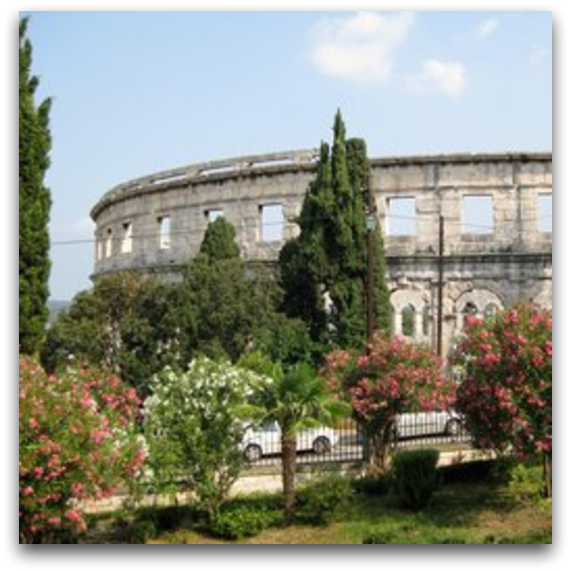
\includegraphics[width=0.33\textwidth]{gfx/source}\label{fig:orig0}}%
  \subfloat[Filtered]{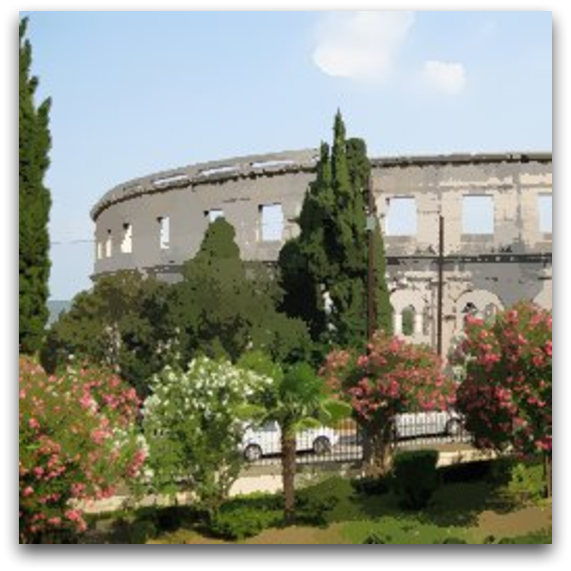
\includegraphics[width=0.33\textwidth]{gfx/filtimage_ref}\label{fig:filt}}%
  \caption{Mean shift filtering with parameters $(h_r, h_f) = (6.5,
    7)$ applied to a color image}
  \label{fig:filtsample}
\end{figure}

The pixels $x_n, n = 1, \ldots, N$ of the image converge toward their
local density maximum applying the filtering \autoref{alg:msf}.

\begin{algorithm2e}[H]
	\DontPrintSemicolon
	\KwData{$x_n=(x_n^r, x_n^f),n=1,\ldots,N$ the $D$-dimensional \gls{RGB} pixels}
	\KwData{$c_n=(c_n^r, c_n^f),n=1,\ldots,N$ the $D$-dimensional \gls{LUV} pixels}
	\KwData{$z_n=(z_n^r, z_n^f),n=1,\ldots,N$ the $D$-dimensional filtered pixels}
	\KwData{$o_n=(o_n^r, o_n^f),n=1,\ldots,N$ the $D$-dimensional output pixels}
	\BlankLine
	
	\For{$n=1, \ldots, N$}{
		convert $x_n$ from \gls{RGB} to \gls{LUV} color space\;
		$c_n = x_n$\;
	}
	\BlankLine
	\For{$n=1, \ldots, N$}{
		initialize $m = 1$ and	$y_n = c_n$\;
		\While{not converged}{
			calculate $y_{n,m+1}$ according to $y_{j+i} = 
		  \frac{\sum_{i=1}^n x_i g\left(\left\lVert \frac{x - x_i}{h}
		      \right\rVert^2\right)}{\sum_{i=1}^n g\left(\left\lVert \frac{x - x_i}{h}
		      \right\rVert^2\right)} $
		}
		assign $z_n = (x_n^r, y_{conv}^f)$\;
	}
	\BlankLine
	\For{$n=1, \ldots, N$}{
		convert $z_n$ from \gls{LUV} to \gls{RGB} color space\;
		$o_n = z_n$\;
	}

	\caption{Mean Shift Filtering}
	\label{alg:msf}
\end{algorithm2e}


All pixels that converge to the same um are lying in the basin of
attraction of this maximum. The filtered image points $z_n, n = 1 ,
\ldots , N$ keep there spatial coordinates but obtain the color values
off the convergence point. The convergence points are found by moving
the kernel window with \emph{mean shift} in direction of maximum slope
of the spatial range feature space. The sample
\autoref{fig:filtsample} was smoothed with the algorithm of
\autoref{alg:msf}.  A uniform kernel with $h = (6.5, 7)$ was used.

\subsection{Mean Shift Segmentation} % (fold)
\label{sub:mean_shift_segmentation}
Image segmentation is a method to partition an image into homogeneous
regions.  Searched are regions with similar colors like a wall, lawn
and clothes.  The found areas are associated with the same color
values. The segmentation can be seen as a strong smoothing where the
edges are preserved.

The segmentation algorithm is a extension of the \emph{mean shift }
filtering algorithm. After applying the filter and all convergence
points are found, clusters are build out of them. All convergence
points that are closer then $h_r$ in the spatial domain and that are
closer then $h_f$ in the range domain are grouped together. In the end
all points are labeled after their cluster assignment.

\begin{figure}[ht]
  \centering \subfloat[Original]{%

    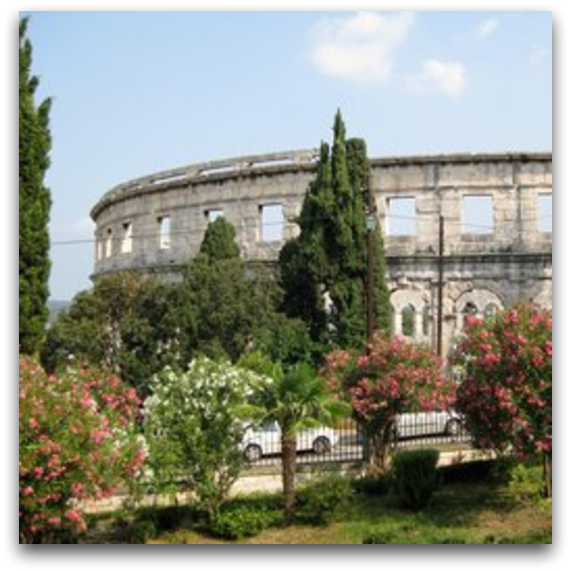
\includegraphics[width=0.33\textwidth]{gfx/source}\label{fig:orig}}%
  \subfloat[Segmented]{%

    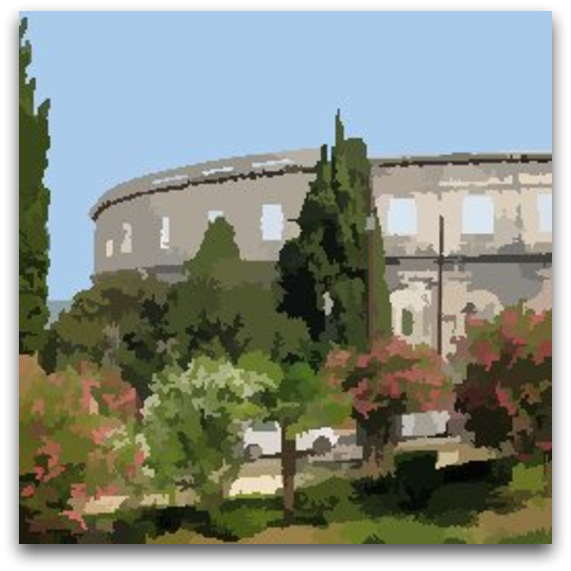
\includegraphics[width=0.33\textwidth]{gfx/segmimage_ref}\label{fig:segm}}%
  \subfloat[Region boundaries]{%

    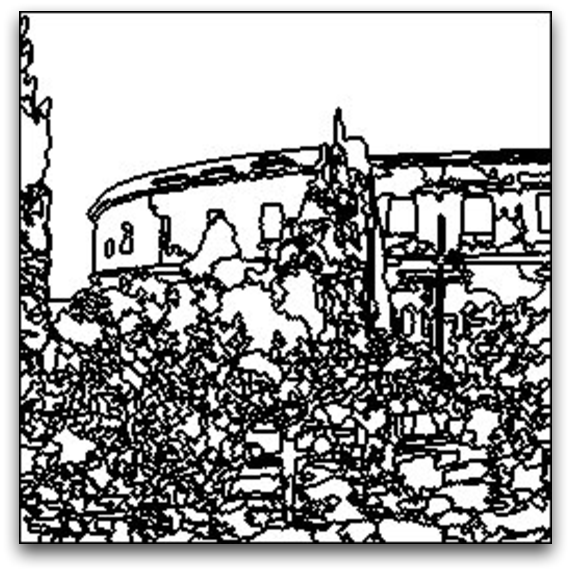
\includegraphics[width=0.33\textwidth]{gfx/bndyimage_ref}\label{fig:bndy}}%

  \caption{Mean shift segmentation with parameters $(h_r, h_f, M) =
    (6.5, 7, 20)$ applied to a color image}
  \label{fig:mssegm}
\end{figure}


The Algorithm was applied on the image \autoref{fig:orig}. A uniform
kernel with a kernel radius of $h_r = 6.5$ and $h_f = 7$ was used. $M$
is a parameter for the last step of the algorithm where regions where
the pixel count is smaller than $M$ are purged. $M$ defines the
smallest significant feature size.  \autoref{fig:mssegm} shows the
result of a segmentation. After the image segmentation follows a edge
detection by examining the cluster regions \autoref{fig:bndy}.

In filtering as well as in segmentation algorithm a fixed sized window
size is used. In \citeauthor{citeulike:462300}
\citep{citeulike:462300} ist is noted that for segmenation the
algorithm is not heavily dependent on the choice of the kernel
parameters where as there are application where the window size
matters.  The segmentation part of the \autoref{alg:mss} has no
significant impact on the run time.


\newcommand{\mycapfn}[1]{\color{black} #1}
%\SetKwSty{mycapfn}

\begin{algorithm2e}[H]
	\DontPrintSemicolon
	\KwData{$x_n=(x_n^r, x_n^f),n=1,\ldots,N$ the $D$-dimensional \gls{RGB} pixels}
	\KwData{$c_n=(c_n^r, c_n^f),n=1,\ldots,N$ the $D$-dimensional \gls{LUV} pixels}
	\KwData{$z_n=(z_n^r, z_n^f),n=1,\ldots,N$ the $D$-dimensional filtered pixels}
	\KwData{$o_n=(o_n^r, o_n^f),n=1,\ldots,N$ the $D$-dimensional output pixels}
	\BlankLine
	

	\For{$n=1, \ldots, N$}{
		convert $x_n$ from \gls{RGB} to \gls{LUV} color space\;
		$c_n = x_n$\;
	}
	\BlankLine
	
	\For{$n=1, \ldots, N$}{
		initialize $m = 1$ and	$y_n = c_n$\;
		\While{not converged}{
			calculate $y_{n,m+1}$ according to $y_{j+i} = 
		  \frac{\sum_{i=1}^n x_i g\left(\left\lVert \frac{x - x_i}{h}
		      \right\rVert^2\right)}{\sum_{i=1}^n g\left(\left\lVert \frac{x - x_i}{h}
		      \right\rVert^2\right)} $
		}
		assign $z_n = (x_n^r, y_{conv}^f)$\;
	}
	\BlankLine
	\For{$n=1, \ldots, N$}{
		delineate in the joint domain the clusters $\{C_p\}_{p=1,\ldots,P}$ by
		grouping together all $z_n$ which are closer than $h_s$ in the spatial 
		domain and $h_r$ in the range domain. 
	}
	\BlankLine
	
	\For{$n=1, \ldots, N$}{
		assign $L_n = \{p|z_i \in C_p\}$\;	
	}
	\BlankLine
	eliminate spatial regions containing less than $M$ pixels\;
	\BlankLine
	\For{$n=1, \ldots, N$}{
		convert $z_n$ from \gls{LUV} to \gls{RGB} color space\;
		$o_n = z_n$\;
	}
	
	\caption{Mean shift segmentation}
	\label{alg:mss}
\end{algorithm2e}



